\documentclass[11pt,a4paper]{article}
\usepackage[latin1]{inputenc}
\usepackage[margin=1in]{geometry}
\usepackage{amsmath}
\usepackage{amsfonts}
\usepackage{amssymb}
\usepackage{graphicx}
\usepackage{enumitem}
\usepackage{listings}
\usepackage{color}

\definecolor{dkgreen}{rgb}{0,0.6,0}
\definecolor{gray}{rgb}{0.5,0.5,0.5}
\definecolor{mauve}{rgb}{0.58,0,0.82}

\lstset{frame=tb,
 language=MatLab,
 aboveskip=3mm,
 belowskip=3mm,
 showstringspaces=false,
 columns=flexible,
 basicstyle={\small\ttfamily},
 numbers=none,
 numberstyle=\tiny\color{gray},
 keywordstyle=\color{blue},
 commentstyle=\color{dkgreen},
 stringstyle=\color{mauve},
 breaklines=true,
 breakatwhitespace=true,
 tabsize=3
}

\setlength\abovedisplayskip{0pt}
\author{James Brissette}
\title{CS-6210: HW 2}
\begin{document}
	\maketitle
	
	\section{Chapter 4}
		\begin{itemize}
			\item[4.22]
				\begin{enumerate} [label={\alph*)}]
					\item I calculated the eigenvalues by hand to be $\frac{1}{\sqrt{3}}$ and $-\frac{1}{\sqrt{3}}$. Using the orthogonal iteration proceedure found in Table 4.9 of the text and with the modified Gram-Schmidt described on page 144, I constructed the following program used for compare my calculated eigenvalues above and consequently for part c below:
					\begin{lstlisting} 
%Orthogonal Iteration Algorithm
function [out] = ch4q22(n)

%Value used to shift
omega = 4;
%Setup matrix A based on input n
A =  zeros(n);
for k=2:n
    A(k-1,k) = (k-1) / sqrt((2*(k-1) - 1)*(2*(k-1) + 1));
    A(k,k-1) = A(k-1,k);
end
As = A - omega*eye(n);

%Randomly select B and calculate preliminary eigenvalues
B = rand(n,n);
Q = GS(B);
eigenvals = zeros(n,1);

eigenvec = Q(:,1);
eigenval = dot(eigenvec, A*eigenvec) / dot(eigenvec, eigenvec);

%Run orthogonal iteration until condition satisfied
iterativeErr = 10000;
while abs(iterativeErr) > 1e-12
    B = As*Q;
    Q = GS(B);
    
    e = eigenval;
    eigenvec = Q(:,1);
    eigenval = dot(eigenvec, As*eigenvec) / dot(eigenvec, eigenvec);
    
    iterativeErr = e - eigenval;
end

%Compute eigenvalues
for k=1:n
    eigenvec = Q(:,k);
    eigenval = dot(eigenvec, As*eigenvec) / dot(eigenvec, eigenvec);
    eigenvals(k) = eigenval + omega;
end

out = eigenvals;
end

%Gram-Schmidt Algorithm
function [Q] = GS(A)
[m,n] = size(A);
e = zeros(m,n);
for j=1:n
    e(:,j) = A(:,j);
    for k=1:j-1
        r = dot(e(:,j),e(:,k)) / dot(e(:,k),e(:,k));
        e(:,j) = e(:,j) - r*e(:,k);
    end
    e(:,j) = e(:,j)/norm(e(:,j));
end

Q = e;
end
					\end{lstlisting}
					\item My approximations of 1 were off by 1.718e-06 in either direction. The exact values were:
					$$1 - 2q_{11}^2 = 1.717584309335329e-06$$
					$$1 - 2q_{21}^2 = -1.717584309446352e-06$$
					
					
					\item Below are the returned eigenvalues of $A$ computed using orthogonal iteration. You'll notice the the values are symmetric, which is a good sign considering the matrix $A$ is also symmetric. Additional confidence comes from knowing the relationship between $tr(A)$ and the sum of the eigenvalues, namely that they should be equal, and in this case, the diagonals are 0 and the eigenvalues symmetric, hinting that our results appear to be valid.
					$$ \lambda_i 's = 
					\begin{pmatrix}
						 -0.9739 \\
   						-0.8651\\
   						-0.6794\\
  						 -0.4334\\
  						 -0.1489\\
  					 	 0.1489\\
   					 	0.4334\\
    					0.6794\\
    					0.8651\\
    					0.9739
					\end{pmatrix}
					$$
					\item Calculating the $\overline{w}_j$'s for each eigenvector resulted in the below vector $w$ where $$w_i = 2q_{j1}^2$$
					$$ w = 
					\begin{pmatrix}
						0.0667 \\
    					0.3355 \\
    					0.0405 \\
    					0.3759 \\
    					0.2300 \\
    					0.2045 \\
    					0.3612 \\
    					0.1445 \\
    					0.2854 \\
    					0.0196
					\end{pmatrix}
					$$
				\end{enumerate}
					
			\item[4.31]
				\begin{enumerate} [label={\alph*)}]
					\item Given $A$, $\lambda_i$, and $x_i$ as below:
					$$A = 
					\begin{pmatrix}
						a & b &      &      &       &    \\
						b & a & c    &      &       &    \\
						  & b & a    & c    &       &    \\
						  &   &\ddots&\ddots&\ddots &    \\
						  &   &      &  b   &   a   & c  \\
						  &   &      &      &   b   & a  &        					
					\end{pmatrix}$$
					$$\lambda_i = a + 2\vert b \vert cos(i\theta) \quad for \quad i=1,2,\dots,n \quad where \quad \theta = \frac{\pi}{n+1}$$
					$$x_i = (sin(\phi) , sin(2\phi),\dots,sin(n\phi)) \quad for \quad \phi = i\theta$$
					If $x_i$ is and eigenvector for the eigenvalue $\lambda_i$, then the following should hold:
					$$(A-\lambda_i I)x_i = 0$$
					Solving for $A-\lambda_i I$ we see that the diagonals $a$ become:
					$$a-(a+ 2\vert b \vert cos(i\theta)) =  -2\vert b \vert cos(i\theta)$$ and we solve:
					$$\begin{pmatrix}
						-2\vert b \vert cos(i\theta) & b & \\
						b & -2\vert b \vert cos(i\theta) & c \\
						  &\ddots&\ddots&\ddots& &\\
						  &   &      b    & -2\vert b \vert cos(i\theta)       					
					\end{pmatrix}
					\begin{pmatrix}
					sin(i\theta) \\
					sin(2i\theta) \\
					sin(3i\theta) \\
					\vdots\\
					sin(ni\theta) \\
					\end{pmatrix} = 
					\begin{pmatrix}
					0\\0\\0\\ \vdots \\ 0
					\end{pmatrix}$$
					
					There are three cases to show this holds true: the two end cases $b+(a-\lambda_i)$ and $(a - \lambda_i) + c$, and the general case in between where $b+(a-\lambda_i)+c$ \\
					\begin{enumerate}
						\item [$(a - \lambda_i) + c$:] ~
						\\ Here we use the trigonometric identity $sin(2x) = sin(x)cos(x)$ and substitute $b$ for $c$ since $b=c$
						$$-2\vert b \vert cos(i\theta)sin(i\theta) + b sin(2i\theta) = 0$$
						$$-\vert b \vert (2sin(i\theta)cos(i\theta)) + b sin(2i\theta) = 0$$
						$$-b(sin(2i\theta)) + b sin(2i\theta) = 0$$
						$$ 0 = 0$$
						
						\item [$b + (a - \lambda_i) + c$:] ~
						\\ Here we use the trigonometric identity $sin(\alpha \pm \beta) = sin(\alpha)cos(\beta) \pm sin(\beta)cos(\alpha)$
						$$bsin(i\theta)-2\vert b \vert cos(i\theta)sin(2i\theta) + b sin(3i\theta) = 0$$
						$$bsin(i\theta)-2\vert b \vert cos(i\theta)sin(2i\theta) + b sin(2i\theta + i\theta) = 0$$
						$$bsin(i\theta)-2\vert b \vert cos(i\theta)sin(2i\theta) + b [sin(2i\theta)cos(i\theta) + sin(i\theta)cos(2i\theta)] = 0$$
						$$bsin(i\theta)-bcos(i\theta)sin(2i\theta) + bsin(i\theta)cos(2i\theta) = 0$$
						$$bsin(i\theta)-b(cos(i\theta)sin(2i\theta) - sin(i\theta)cos(2i\theta)) = 0$$
						$$bsin(i\theta)-bsin(2i\theta - i\theta) = 0$$
						$$ 0 = 0$$
						
						\item [$b + (a - \lambda_i)$:] ~
						\\ Here we use the trigonometric identity $sin(\alpha \pm \beta) = sin(\alpha)cos(\beta) \pm sin(\beta)cos(\alpha)$
						$$bsin((n-1)i\theta)-2\vert b \vert cos(i\theta)sin(ni\theta) = 0$$
						$$bsin(ni\theta - i\theta)-2\vert b \vert cos(i\theta)sin(ni\theta) = 0$$
						$$b[sin(ni\theta)cos(i\theta)-sin(i\theta)cos(ni\theta)]-2\vert b \vert cos(i\theta)sin(ni\theta) = 0$$
						$$-b(sin(ni\theta)cos(i\theta)- bcos(ni\theta)sin(i\theta) = 0$$
						$$-b[sin(ni\theta)cos(i\theta) + cos(ni\theta)sin(i\theta)] = 0$$
						$$-bsin((n+1)i\theta) = 0$$
						$$-bsin(\frac{(n+1)i\pi}{n+1}) = 0$$
						$$-bsin(i\pi) = 0$$
						$$ 0 = 0$$
							
					\end{enumerate}
					\item Because $cos(i\theta)$ simply oscillates between -1 and 1, we have in the worst case that $cos(i\theta)=-1$. Because the problem posits that $\lambda_i=a+2\vert b \vert cos(i\theta)$ and we are given that $a\geq 2\vert b \vert$, we see that in the worst case that $cos(i\theta) = -1$ and $a$ is no bigger than $2\vert b \vert$:
					$$a + 2\vert b \vert (-1)$$
					$$a-2\vert b \vert$$
					$$2\vert b \vert-2\vert b \vert = 0 $$
					This does two things. First, it precludes the matrix $A$ from being classified as \textit{strictly diagonally dominant} since it is not strictly greater than the sum of the other elements in it's row (the first method I tried of proving positive definiteness), so we can't prove it that way. Second, it shows that by Theorem 3.1 we fail altogether in proving positive definiteness in that we can't prove that $A$ has only positive eigenvalues. Without the constraint the $a \geq 2\vert b \vert$ tightened to $a > 2\vert b \vert$ we can only prove semi-positive definiteness.
					\item Because $A$ is symmetric, according to Theorem 4.1, if $x_i$ and $x_j$ are eigenvectors for different eigenvalues (as we proved in part a), then: $x_i \bullet x_j = 0$\\
					Additionally, to show $x_i \bullet x_i = \frac{n+1}{2}$ we use the trigonometric identity $sin^2(x) = \frac{1}{2}(1- cos(2x))$
					$$ x_i \bullet x_i = sin^2(i\theta)+sin^2(2i\theta)+\dots + sin^2(ni\theta)$$
					$$= \frac{1}{2}(1- cos(2i\theta))+\frac{1}{2}(1- cos(4i\theta))+\dots + \frac{1}{2}(1- cos(2nix))$$
					$$= \frac{(1- cos(2i\theta))+(1- cos(4i\theta))+\dots + (1- cos(2nix))}{2}$$
					$$= \frac{n - \Sigma_{k=1}^n cos(\frac{2ki\pi}{n+1})}{2}$$
					\begin{center}
						As it turns out because cosine has a period of $2\pi$ that $\forall n \geq 3 \quad \Sigma_{k=1}^n cos(\frac{2ki\pi}{n+1}) = -1$
					\end{center}
					$$ x_i \bullet x_i = \frac{n - \Sigma_{k=1}^n cos(\frac{2ki\pi}{n+1})}{2} = \frac{n+1}{2}$$
					\item Taking a look at the new $\lambda_i$ we see in interesting coincidence stemming from the symmetry of the matrix, namely that $b=c$ so in substituting back into $$\lambda_i = a+2\sqrt{bc}cos(i\theta) = a + 2\sqrt{b^2}cos(i\theta) = a + 2bcos(i\theta)$$ From part a we determined $\lambda_i = a + 2bcos(i\theta)$ assuming $b > 0$ and in part c we solved $\lambda_i = a + 2bcos(i\theta)$ for $b=c$.\\
					Turning our attention to the additional constraint $\kappa=\sqrt{\frac{b}{c}}$ again we see that due to the symmetric nature of $A$, $b=c$ and $\kappa=\sqrt{\frac{b}{b}} = \sqrt{1} = 1$. Substituting this back into $x_i$ we see the structure has not changed from that of part $a$ in that:
					$$x_i = (\kappa sin(\phi), \kappa^2 sin(2\phi), \dots, \kappa^n sin(n\phi)$$
					$$x_i = (1 sin(\phi), 1^2 sin(2\phi), \dots, 1^n sin(n\phi)$$
					$$x_i = (sin(\phi),sin(2\phi), \dots,sin(n\phi))$$
					And in part a we proved that $x_i$ is an eigenvector for $\lambda_i$ if the same conditions held true.
				\end{enumerate}
		\end{itemize}
		
	\section{Chapter 9}
		\begin{itemize}
			\item[9.2]
				\begin{enumerate} [label={\alph*)}]
					\item The result of the normalization using $\overline{X}=2.8215$, $\overline{Y}=2.4224$, and scaling $X$ by $7.1118$ and $Y$ by $2.0859$ is:
						$$\begin{array}{cc}
							p & q \\ \hline
							-1.0000  & 0.5963 \\
							-0.8151  & 0.6407 \\
							-0.6096  & 0.2867 \\
							-0.3397  & 0.5540 \\
							-0.1761  & 0.4480 \\
							0.2006 & -0.1704 \\
							0.2508  & 0.0572 \\
							0.4053   & -0.0117 \\
							0.5854  & -0.5213 \\
							0.6720  & -0.8795 \\
							0.8265  & -1.0000 \\
							
						
						\end{array}$$
					\item The $\alpha$ calculated using the normalized table in part a: $$\alpha = -0.9281$$
					\item Since we have $G(X)=V_1 + V_2 X$ where $G(X)$ is a linear function with slope $V_2$, it follows that $m=V_2=v_2$ and for the analogous function $Y$,
					$$Y=\overline{Y} + m(X-\overline{X})$$
					Rearranging Y we group the constants and get:
					$$Y=(\overline{Y}-m\overline{X})+mX$$ Since $V_1=log(v_1)$, we can solve for $v_1$ as:
					$$V_1= log(v_1)=\overline{Y}-m\overline{X}$$
					$$v_1=10^{\overline{Y}-m\overline{X}}$$
					\item
						\begin{center}
							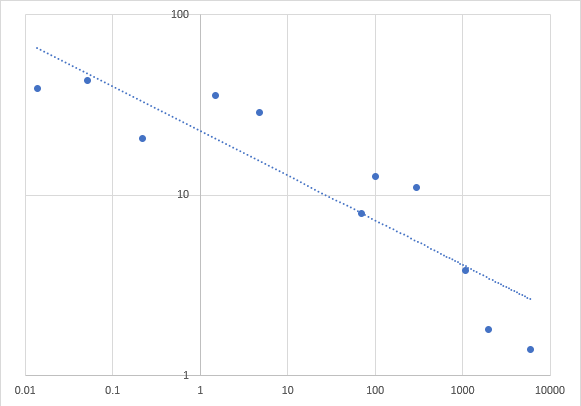
\includegraphics[width=0.7\linewidth]{plot}
						\end{center}
					\item Based on the data, and a thorough Google search of T-Rex massses, they tend to be in the range of 13e03 to 32e03 kg. Estimating the speed of a slightly heavier T-Rex with a mass of $\approx 20,000kg$ we get a speed of about 10.79814949 (converting back to standard metric).
 
				\end{enumerate}
					
			\item[9.3]
				\begin{enumerate} [label={\alph*)}]
					\item Given $ZZ^T = \frac{1}{n} \Sigma_{i=1}^{n} s_i(s_i)^T$ and $s_i^* = Z^{-1}s_i$ we can plug into 9.30 and get back the original $ZZ^T$ as follows:
					\begin{equation}
						\frac{1}{n} \Sigma_{i=1}^{n} s_i^*(s_i^*)^T = I
					\end{equation}
					\begin{equation}
						\frac{1}{n} \Sigma_{i=1}^{n} Z^{-1}s_i(Z^{-1}s_i)^T = I
					\end{equation}
					\begin{equation}
						\frac{1}{n} \Sigma_{i=1}^{n} Z^{-1}s_i (s_i)^T (Z^{-1})^{T}= I
					\end{equation}
					\begin{equation}
						Z^{-1} (\frac{1}{n} \Sigma_{i=1}^{n} s_i (s_i)^T) (Z^{-1})^{T}= I
					\end{equation}
					\begin{equation}
						ZZ^{-1} (\frac{1}{n} \Sigma_{i=1}^{n} s_i (s_i)^T) (Z^{-1})^{T}Z^T= ZIZ^T
					\end{equation}
					\begin{equation}
						\frac{1}{n} \Sigma_{i=1}^{n} s_i(s_i)^T = ZZ^T
					\end{equation}
					
					\setcounter{equation}{0}
					\item For this problem we will show that given $\frac{1}{n} \Sigma_{i=1}^{n} s_i(s_i)^T = U \Sigma U^T$ and $s_{i}^{*} = \Sigma^{-\frac{1}{2}} U^T s_i$ we can plug $s_i^*$ into 9.30 and get back the identity matrix $I$:
						\begin{equation}
							\frac{1}{n} \Sigma_{i=1}^{n} s_i^*(s_i^*)^T = I
						\end{equation}
						\begin{equation}
							\frac{1}{n} \Sigma_{i=1}^{n} (\Sigma^{-\frac{1}{2}} U^T s_i)(\Sigma^{-\frac{1}{2}} U^T s_i)^T = I
						\end{equation}
						\begin{equation}
							\frac{1}{n} \Sigma_{i=1}^{n} (\Sigma^{-\frac{1}{2}} U^T s_i)(s_i^T  U^{T^T}  \Sigma^{-\frac{1}{2}T}) = I
						\end{equation}
						\begin{equation}
							\Sigma^{-\frac{1}{2}}U^T (\frac{1}{n} \Sigma_{i=1}^{n} s_i(s_i^T))U\Sigma^{-\frac{1}{2}T} = I
						\end{equation}
						\begin{equation}
							\Sigma^{-\frac{1}{2}}U^T (U \Sigma U^T) U\Sigma^{-\frac{1}{2}T} = I
						\end{equation}
						\begin{equation}
							\Sigma^{-\frac{1}{2}}(\Sigma )\Sigma^{-\frac{1}{2}T} = I
						\end{equation}
						And since we know $\Sigma$ is a diagonal matrix:
						\begin{equation}
							I = I
						\end{equation}
						
					\item For the first matrix, after centering the data, we find that plugging it into the summation gives us a new matrix: $$\begin{pmatrix}
						1 & -1 \\
						-1 & 1					
					\end{pmatrix}$$
					If we select $Z$ to be equal to the below:
					$$Z=\frac{1}{\sqrt{2}}
					\begin{pmatrix}
						1 & -1 \\
						-1 & 1					
					\end{pmatrix}$$ then we satisfy the condition $$ZZ^T = \frac{1}{n} \Sigma_{i=1}^{n} s_i(s_i)^T = \begin{pmatrix}
						1 & -1 \\
						-1 & 1					
					\end{pmatrix}$$ However, this $Z$ is not invertible and so we can't use it to whiten the data. Exploring other options we see that there's no other immediately obvious answer given that $Z$ is not unique (per the text).				
					
 				\end{enumerate}
				
			\item[9.5]
				\begin{enumerate} [label={\alph*)}]
					\item Since we have that $p = \alpha_1 v_1$ we can decompose the vector $p$ into its two parts, namely $p_1$ and $p_2$ which correspond to the first and second entries of $v_1$ times some scaling factor $\alpha_1$:
					$$\begin{pmatrix} p_1 \\ p_2 \end{pmatrix}= \alpha_1 \begin{pmatrix} v_{11} \\ v_{21} \end{pmatrix}$$
					$$p_1 = \alpha_1 v_{11} \quad p_2 = \alpha_1 v_{21}$$
					Solving for $\alpha_1$ in the first equation we get that $\alpha_1=\frac{p_1}{v_{11}}$ and substituting into the equation for $p_2$ we see:
					$$p_2 = \alpha_1 v_{21} = \frac{v_{21}}{v_{11}}p_1 \quad where \quad \alpha_1 = \frac{v_{21}}{v_{11}}$$
					\item Since in part $a$ we saw that $p_2 = \alpha p_1$ we can use the fact that the variables $p_1$ and $p_2$ are the normalized versions of $q_1$ and $q_2$ (namely that they are centered and scaled) to derive the equation that relates them:
					$$p_1 = \frac{1}{S_1}(q_1 - M_1), \quad p_2 = \frac{1}{S_2}(q_2 - M_2)$$
					$$p_2 = \frac{1}{S_2}(q_2 - M_2) = \alpha p_1 = \alpha \frac{1}{S_1}(q_1 - M_1)$$
					$$\frac{1}{S_2}(q_2 - M_2) = \alpha \frac{1}{S_1}(q_1 - M_1)$$
					$$q_2 - M_2 = \frac{\alpha S_2}{S_1}(q_1 - M_1) \quad where \quad a = \frac{\alpha S_2}{S_1}$$
					$$q_2 = M_2 + a(q_1 - M_1)$$
				\end{enumerate}
				
			\item[9.8]
				\begin{enumerate} [label={\alph*)}]
					\item Included for reference below is the code used to generate the below times for each part of the question. \\ Below is one reference table for the calculated times for each test and each run time:
					$$\begin{array}{ccc}
						       & Size & Times \\ \hline
						Part A & 2000    & 3.607285975884664e-03 \\
						       & 20000   & 3.317933575600404e-02 \\
						       & 200000  & 3.302640852477376e-01 \\
						       &         &						 \\
						Part B & 2000    & 3.758302269764120e-04 \\
						       & 20000   & 3.413897520502541e-03 \\
						       & 200000  & 3.592276018280914e-02 \\
						       &         &						 \\
						Part C & 2000    & 3.826568492037185e-04 \\
						       & 20000   & 3.482651358648984e-03 \\
						       & 200000  & 3.866706231818633e-02 \\
						       &         &						 \\
						Part D & 2000    & 4.195206092311732e-04 \\
						       & 20000   & 3.526829356777124e-03 \\
						       & 200000  & 4.035226277658426e-02 
		
					\end{array}$$
					\item Right off the bat I noticed that for each order of magnitude increase in the size, there was a proportional increase in the time to compute. Parts B, C, and D were all faster than part A, however, they appeared to slow down as the tests progressed (e.g. D was slower than C was slower than B). This may be due to my implementation, or may be a system nuance. In any case, the difference in computing time was not super large and may not be as pronounced without a significantly larger dataset.
					\\
					\begin{lstlisting}
function [out] = ch9q8()

len1 = 2000;
len2 = 20000;
len3 = 200000;

x1 = rand(2,len1);
x2 = rand(2,len2);
x3 = rand(2,len3);

%n=2000
x1a = @() summation(x1,len1);
time_x1a = timeit(x1a);

x1b = @() centersum(x1,len1);
time_x1b = timeit(x1b);

x1c = @() cstars(x1,len1);
time_x1c = timeit(x1c);

x1d = @() callCov(x1,len1);
time_x1d = timeit(x1d);


%n=20000
x2a = @() summation(x2,len2);
time_x2a = timeit(x2a);

x2b = @() centersum(x2,len2);
time_x2b = timeit(x2b);

x2c = @() cstars(x2,len2);
time_x2c = timeit(x2c);

x2d = @() callCov(x2,len2);
time_x2d = timeit(x2d);


%n=200000
x3a = @() summation(x3,len3);
time_x3a = timeit(x3a);

x3b = @() centersum(x3,len3);
time_x3b = timeit(x3b);

x3c = @() cstars(x3,len3);
time_x3c = timeit(x3c);

x3d = @() callCov(x3,len3);
time_x3d = timeit(x3d);

disp('Times:')
disp('Part A, n=2000')
disp(time_x1a)
disp('Part B, n=2000')
disp(time_x1b)
disp('Part C, n=2000')
disp(time_x1c)
disp('Part D, n=2000')
disp(time_x1d)
disp('%%%%%%%%%%%%%%%%%%%%%%%')
disp('Part A, n=20000')
disp(time_x2a)
disp('Part B, n=20000')
disp(time_x2b)
disp('Part C, n=20000')
disp(time_x2c)
disp('Part D, n=20000')
disp(time_x2d)
disp('%%%%%%%%%%%%%%%%%%%%%%%')
disp('Part A, n=200000')
disp(time_x3a)
disp('Part B, n=200000')
disp(time_x3b)
disp('Part C, n=200000')
disp(time_x3c)
disp('Part D, n=200000')
disp(time_x3d)
end

function [out] = calculateCenter(in)
    [m,n] = size(in);
    out = in;
    avg = mean(out);
    for k=1:n
        out(:,k) = out(:,k) - avg(k);
    end
end

function summation(x,n)

xc = calculateCenter(x);
B = zeros(2,2);
for k=1:n
    vec = xc(:,k);
    B = B + (vec*vec');
end
B = B / n;
end

function centersum(x,n)

xc = calculateCenter(x);
B = (xc*xc')/n;

end

function cstars(x,n)

xc = calculateCenter(x);
cstar1 = xc(1,:)';
cstar2 = xc(2,:)';

B = dot(cstar1,cstar2)/n;

end

function callCov(x,n)

xc = calculateCenter(x);
B = cov(xc');

end
					\end{lstlisting}
				\end{enumerate}
		\end{itemize}
		
	
\end{document}